\subsection{Degree dependent layer combination}\label{subsec:degree-experiment}
In this experiment we investigated how the nodes within a certain range of node degree perform.
The node degree is the number of connections the node has in the original interaction graph.
Our initial hypothesis was that the fewer connections a node had, the more it would benefit from a higher number of convolutions.
However the results obviously confirm that this is not the case.
We answer the following research question in this section:
\begin{itemize}
    \item \textbf{RQ4}: Is it beneficial to change layer combination based on the degree of the nodes?
\end{itemize}

\subsubsection{Only utilizing one layer}
To be able to test ALC and BLC on different node degree ranges, we first had to find out how the different node degree ranges performed when only using one layer.
The NDCG results can be seen for Amazon-Cell-Sport on \autoref{tab:Amazon-Cell-Sport-ndcg-evaluation} and \autoref{fig:ndcg-individual-evaluation-amazon-book}, Yelp2020 on \autoref{tab:yelp2020-ndcg-evaluation} and \autoref{fig:yelp2020-ndcg-individual-evaluation} and Amazon-Book on \autoref{tab:amazon-book-NDCG-evaluation} and \autoref{fig:amazon-cell-sport-individual-evaluation-ndcg}.
The results have been evaluated within a certain node degree, and "Combined" is where all nodes have been evaluated together to get the overall performance.
The rightmost column is the result of the best performing original LightGCN method.
All of the results for LightGCN with different layers can be found in Appendix \ref{app:average-lightgcn-results}.
The tables and figures containing the results of the recall performance for the different degree ranges can be found in Appendix \ref{app:individual-recall-degree-experiment}.
The experiments with the Amazon-Cell-Sport dataset can be seen on \autoref{tab:Amazon-Cell-Sport-ndcg-evaluation}.
These results showcase that for nodes with less than 46 connections $E^{(5)}$ is usually the best performing embedding and for nodes with more than 46 connections $E^{(5)}$ performs worse than other embeddings with a lower number of convolutions.
$E^{(5)}$ does however often perform second best for many node degree ranges.
It is also worth noting that $E^{(3)}$, $E^{(4)}$ and $E^{(5)}$ consistently outperform LightGCN with 5 convolutions.
This could be because utilizing $E^{(0)}$ and $E^{(1)}$ is harmful for performance, because 91 \% of all items only have between 1-5 connections and therefore the embeddings need more convolution to capture the collaborative signals.
Looking at the yelp2020 and amazon-book datasets seen on \autoref{tab:yelp2020-ndcg-evaluation} and \autoref{tab:amazon-book-NDCG-evaluation} the results do not seem to be dependent on the degree of the nodes, as almost all node degree ranges either perform best or second best in $E^{(1)}$ and $E^{(2)}$.
In both of these datasets nodes have above 19 connections on average and therefore the amount of collaborative signals increase much faster for each node in the graph compared to amazon-cell-sport.
For Amazon-Cell-Sport the recall performance increases for the nodes with a higher degree, however for Yelp2020 and Amazon-Book the performance decreases for higher node degrees.
This could be because the nodes with many connections get too much noise in Yelp2020 and Amazon-Book, but for Amazon-Cell-Sport there are many items with few connected users, and hereby it limits how much information users with many connections gain.
The best result for "Combined" in Amazon-Book is 3 convolution with average.
$E^{(1)}$ and $E^{(2)}$ significantly outperform the other embedding layers.
For Yelp2020 the 5 convolution average performs best, while the $E^{(1)}$, $E^{(2)}$ and $E^{(3)}$ embedding layer are the best individual performing layer.
For Amazon-Cell-Sport $E^{(2)}$, $E^{(3)}$, $E^{(4)}$ and $E^{(5)}$ outperform the 5 convolution average.
\\
From these results we see an opportunity to change the layer combination in different ways to investigate if this will improve the results.
The last method is to use \autoref{fredsplit} method to optimize the hyper parameters.
As no direct link between the number of connections a user has and its performance was found, it could be interesting to look further into the number of implicit connections a user has once the convolutions have been performed.
The conclusion on the results are that the individual degree of a node has a smaller effect on the final result than we initially expected.

% Yelp2020 NDCG
\begin{table*}[]
    \centering
    \begin{tabular}{|l|l|l|l|l|l|l||l|}
        \hline
        Node degree & \multicolumn{1}{c|}{$E^{(0)}$} & \multicolumn{1}{c|}{$E^{(1)}$} & \multicolumn{1}{c|}{$E^{(2)}$} & \multicolumn{1}{c|}{$E^{(3)}$} & \multicolumn{1}{c|}{$E^{(4)}$} & \multicolumn{1}{c||}{$E^{(5)}$} & \multicolumn{1}{c|}{5 con} \\ \hline
        6-10        & 0.07550                        & \underline{0.09271}            & 0.09136                        & 0.09211                        & 0.08228                        & 0.07408                         & \textbf{0.10095}           \\ \hline
        11-15       & 0.07677                        & \underline{0.09607}            & 0.09444                        & 0.09531                        & 0.08449                        & 0.07642                         & \textbf{0.10408}           \\ \hline
        16-20       & 0.08704                        & \underline{0.1069}             & 0.10575                        & 0.1043                         & 0.09354                        & 0.08562                         & \textbf{0.11451}           \\ \hline
        21-25       & 0.09096                        & \underline{0.1104}             & 0.10892                        & 0.1066                         & 0.09455                        & 0.08720                         & \textbf{0.11790}           \\ \hline
        26-30       & 0.08578                        & \underline{0.1137}             & 0.10933                        & 0.1092                         & 0.1000                         & 0.09431                         & \textbf{0.11909}           \\ \hline
        31-35       & 0.09420                        & 0.1196                         & \underline{0.12151}            & 0.1151                         & 0.1021                         & 0.09489                         & \textbf{0.12833}           \\ \hline
        36-40       & 0.09886                        & \underline{0.1195}             & 0.11764                        & 0.1108                         & 0.09965                        & 0.09326                         & \textbf{0.12711}           \\ \hline
        41-45       & 0.09512                        & 0.1071                         & \underline{0.11056}            & 0.1049                         & 0.09713                        & 0.09181                         & \textbf{0.11638}           \\ \hline
        46-50       & 0.09113                        & \underline{0.1162}             & 0.11447                        & 0.1147                         & 0.1057                         & 0.1011                          & \textbf{0.12537}           \\ \hline
        51-60       & 0.09782                        & 0.1095                         & \underline{0.11560}            & 0.1128                         & 0.1059                         & 0.1048                          & \textbf{0.12459}           \\ \hline
        61-70       & 0.09618                        & 0.1133                         & \underline{0.11338}            & 0.1125                         & 0.1024                         & 0.09921                         & \textbf{0.12377}           \\ \hline
        71-80       & 0.1067                         & \underline{0.1251}             & 0.12072                        & 0.1145                         & 0.1096                         & 0.1067                          & \textbf{0.13007}           \\ \hline
        81-90       & 0.09104                        & 0.1019                         & \underline{0.10477}            & 0.09683                        & 0.09489                        & 0.09547                         & \textbf{0.11042}           \\ \hline
        91-100      & 0.1045                         & \underline{0.1334}             & 0.13189                        & 0.1303                         & 0.1177                         & 0.1157                          & \textbf{0.14010}           \\ \hline
        101-150     & 0.09488                        & 0.1168                         & \underline{0.11731}            & 0.1142                         & 0.1077                         & 0.1092                          & \textbf{0.12676}           \\ \hline
        151-200     & 0.08451                        & 0.1066                         & \underline{0.11441}            & 0.1117                         & 0.1065                         & 0.1133                          & \textbf{0.11889}           \\ \hline
        201-250     & \textbf{0.1231}                & \underline{0.1217}             & 0.11866                        & 0.1009                         & 0.09105                        & 0.09490                         & \textbf{0.11999}           \\ \hline
        251-300     & 0.2238                         & 0.2224                         & 0.17787                        & 0.2538                         & 0.2806                         & \textbf{0.2917}                 & 0.21693                    \\ \hline
        301+        & 0.1752                         & 0.1989                         & \underline{0.21585}            & 0.2093                         & 0.1719                         & 0.1880                          & \textbf{0.23305}           \\ \hline
        Combined    & 0.08177                        & 0.1019                         & \underline{0.1086}             & 0.09956                        & 0.08863                        & 0.0819                          & \textbf{0.1089}            \\ \hline
    \end{tabular}
    \caption{NDCG@50 for Yelp2020 where only one convolution layer is used and compared with the best performing LightGCN convolution for Yelp2020.}
    \label{tab:yelp2020-ndcg-evaluation}
\end{table*}

\begin{figure}[]
    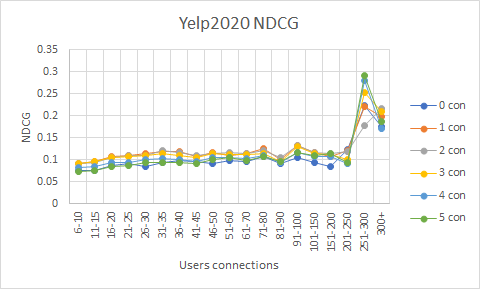
\includegraphics[width=0.5\textwidth]{figures/evaluation/yelp-ndcg-evaluation.png}
    \centering
    \caption{NDCG performance for the individual embedding layers on Yelp2020}
    \label{fig:yelp2020-ndcg-individual-evaluation}
\end{figure}

% Amazon-book
\begin{table*}[]
    \centering
    \begin{tabular}{|l|l|l|l|l|l|l||l|}
        \hline
        Node degree & \multicolumn{1}{c|}{$E^{(0)}$} & \multicolumn{1}{c|}{$E^{(1)}$} & \multicolumn{1}{c|}{$E^{(2)}$} & \multicolumn{1}{c|}{$E^{(3)}$} & \multicolumn{1}{c|}{$E^{(4)}$} & \multicolumn{1}{c|}{$E^{(5)}$} & \multicolumn{1}{c|}{3 con} \\ \hline
        16-20       & 0.03965                        & \underline{0.04851}            & 0.04722                        & 0.03762                        & 0.03287                        & 0.02911                        & \textbf{0.04929}           \\ \hline
        21-25       & 0.03903                        & \textbf{0.04862}               & 0.04807                        & 0.03788                        & 0.03323                        & 0.02964                        & \underline{0.04831}        \\ \hline
        26-30       & 0.03767                        & \textbf{0.04751}               & 0.04624                        & 0.03755                        & 0.03335                        & 0.03014                        & \textbf{0.04778}           \\ \hline
        31-35       & 0.03772                        & \textbf{0.04873}               & 0.04728                        & 0.03865                        & 0.03434                        & 0.03163                        & \underline{0.04825}        \\ \hline
        36-40       & 0.03412                        & \textbf{0.04506}               & \underline{0.04495}            & 0.03730                        & 0.03227                        & 0.02911                        & 0.04493                    \\ \hline
        41-45       & 0.03597                        & \textbf{0.04391}               & 0.04282                        & 0.03607                        & 0.03218                        & 0.02916                        & \underline{0.04301}        \\ \hline
        46-50       & 0.03436                        & 0.04350                        & \textbf{0.04413}               & 0.03784                        & 0.03357                        & 0.03111                        & \underline{0.04368}        \\ \hline
        51-60       & 0.03273                        & \underline{0.04205}            & 0.04077                        & 0.03380                        & 0.02959                        & 0.02719                        & \textbf{0.04210}           \\ \hline
        61-70       & 0.03214                        & \textbf{0.04109}               & \underline{0.04054}            & 0.03401                        & 0.03117                        & 0.02972                        & 0.03972                    \\ \hline
        71-80       & 0.03135                        & \textbf{0.03986}               & \underline{0.03958}            & 0.03445                        & 0.03160                        & 0.02981                        & 0.03923                    \\ \hline
        81-90       & 0.02832                        & \underline{0.03567}            & \textbf{0.03624}               & 0.03140                        & 0.02928                        & 0.02747                        & 0.03551                    \\ \hline
        91-100      & 0.02885                        & \underline{0.03814}            & \textbf{0.03882}               & 0.03163                        & 0.02884                        & 0.02717                        & 0.03781                    \\ \hline
        101-150     & 0.02675                        & \textbf{0.03351}               & 0.03332                        & 0.02927                        & 0.02652                        & 0.02522                        & \underline{0.03334}        \\ \hline
        151-200     & 0.02594                        & \underline{0.03037}            & \textbf{0.03049}               & 0.02728                        & 0.02518                        & 0.02423                        & 0.02932                    \\ \hline
        201-250     & 0.02613                        & 0.03228                        & \textbf{0.03312}               & 0.03096                        & 0.02925                        & 0.02914                        & \underline{0.03242}        \\ \hline
        251-300     & 0.03153                        & \textbf{0.03682}               & 0.03492                        & 0.03594                        & 0.03508                        & 0.03581                        & \underline{0.03617}        \\ \hline
        301+        & 0.03219                        & 0.03874                        & \textbf{0.04227}               & 0.04137                        & 0.04169                        & \underline{0.04207}            & 0.04130                    \\ \hline
        Combined    & 0.03669                        & \underline{0.0458}             & 0.04487                        & 0.0372                         & 0.03247                        & 0.02923                        & \textbf{0.04668}           \\ \hline
    \end{tabular}
    \caption{NDCG@50 for Amazon-Book}
    \label{tab:amazon-book-NDCG-evaluation}
\end{table*}
\begin{figure}[]
    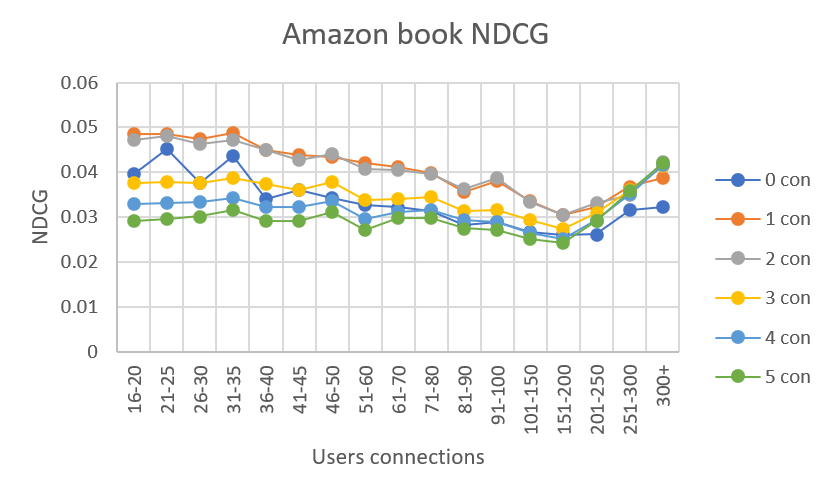
\includegraphics[width=0.5\textwidth]{figures/evaluation/amazon-book-ndcg.png}
    \centering
    \caption{NDCG performance for the individual embedding layers on Amazon-Book}
    \label{fig:ndcg-individual-evaluation-amazon-book}
\end{figure}

% Amazon-Cell-sport NDCG
\begin{table*}[]
    \centering
    \begin{tabular}{|l|l|l|l|l|l|l||l|}
        \hline
        Node degree & \multicolumn{1}{c|}{$E^{(0)}$} & \multicolumn{1}{c|}{$E^{(1)}$} & \multicolumn{1}{c|}{$E^{(2)}$} & \multicolumn{1}{c|}{$E^{(3)}$} & \multicolumn{1}{c|}{$E^{(4)}$} & \multicolumn{1}{c||}{$E^{(5)}$} & \multicolumn{1}{c|}{5 con} \\ \hline
        6-10        & 0.00995                        & 0.02156                        & 0.02250                        & 0.02173                        & \textbf{0.02441}               & \underline{0.02355}             & 0.01972                    \\ \hline
        11-15       & 0.01814                        & 0.02845                        & 0.02901                        & 0.02986                        & \underline{0.03154}            & \textbf{0.03376}                & 0.02984                    \\ \hline
        16-20       & 0.02378                        & 0.03269                        & 0.03737                        & \underline{0.03739}            & 0.03674                        & \textbf{0.03923}                & 0.03701                    \\ \hline
        21-25       & 0.03508                        & 0.04174                        & 0.04424                        & 0.04620                        & \underline{0.04727}            & \textbf{0.04907}                & 0.04438                    \\ \hline
        26-30       & 0.03584                        & 0.04281                        & 0.04606                        & 0.04663                        & \underline{0.04928}            & \textbf{0.04967}                & 0.04815                    \\ \hline
        31-35       & 0.05091                        & 0.06659                        & \textbf{0.07622}               & 0.06981                        & 0.07514                        & \underline{0.07544}             & 0.07514                    \\ \hline
        36-40       & 0.04884                        & 0.05221                        & \underline{0.06001}            & 0.05867                        & 0.05855                        & \textbf{0.06266}                & 0.05475                    \\ \hline
        41-45       & 0.6337                         & 0.07144                        & 0.07698                        & 0.07592                        & \underline{0.08052}            & \textbf{0.08197}                & 0.07634                    \\ \hline
        46-50       & 0.09049                        & 0.10755                        & \textbf{0.11442}               & 0.1030                         & 0.1067                         & \underline{0.1083}              & 0.10074                    \\ \hline
        51-60       & 0.05128                        & 0.07620                        & 0.08498                        & 0.09005                        & \textbf{0.1005}                & \underline{0.09309}             & 0.08827                    \\ \hline
        61-70       & 0.07796                        & 0.08878                        & 0.08324                        & 0.08425                        & \textbf{0.09537}               & \underline{0.09270}             & 0.07718                    \\ \hline
        71-80       & 0.04767                        & 0.05050                        & 0.05611                        & \textbf{0.05930}               & 0.05158                        & 0.05406                         & \underline{0.05834}        \\ \hline
        81-90       & 0.03265                        & 0.07549                        & 0.06440                        & 0.06200                        & \textbf{0.08332}               & \underline{0.08163}             & 0.07351                    \\ \hline
        91-100      & 0.06619                        & 0.07376                        & 0.07435                        & \textbf{0.09016}               & 0.08820                        & 0.08012                         & \underline{0.08968}        \\ \hline
        101-150     & 0.08542                        & 0.11063                        & \textbf{0.11732}               & 0.1151                         & 0.1130                         & \underline{0.1156}              & 0.11290                    \\ \hline
        151-200     & 0.07992                        & 0.08619                        & \textbf{0.10778}               & 0.08642                        & 0.09375                        & 0.08577                         & \underline{0.09668}        \\ \hline
        201-250     & 0.0                            & 0.0                            & 0.0                            & 0.0                            & 0.0                            & 0.0                             & 0.0                        \\ \hline
        251-300     & 0.0                            & 0.0                            & 0.0                            & 0.0                            & 0.0                            & 0.0                             & 0.0                        \\ \hline
        300+        & 0.11521                        & 0.16210                        & 0.12260                        & \underline{0.1752}             & \textbf{0.1786}                & 0.1680                          & 0.16771                    \\ \hline
        Combined    & 0.02169                        & 0.02523                        & 0.03419                        & 0.03483                        & \underline{0.0366}             & \textbf{0.03733}                & 0.03285                    \\ \hline
    \end{tabular}
    \caption{NDCG@50 for Amazon-Cell-Sport where only one convolution layer is used.}
    \label{tab:Amazon-Cell-Sport-ndcg-evaluation}
\end{table*}
\begin{figure}[]
    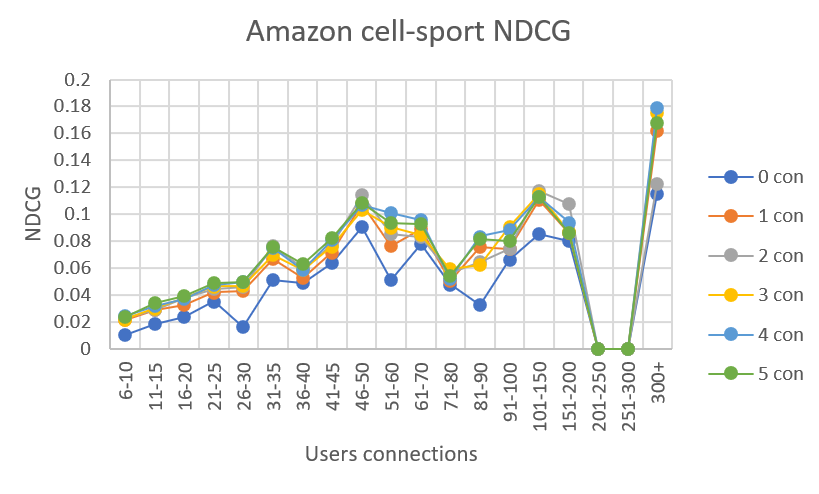
\includegraphics[width=0.5\textwidth]{figures/evaluation/amazon-cell-sport-ndcg.png}
    \centering
    \caption{NDCG performance for the individual embedding layers on Amazon-Cell-Sport}
    \label{fig:amazon-cell-sport-individual-evaluation-ndcg}
\end{figure}

\subsubsection{Degree dependent ALC and BLC}
\todo{Finish writing when Amazon-Book is done.}
Another opportunity for layer combination is to use ALC or BLC based on the node degree.
So instead of using the combined performance results from each layer, then use the results within a certain split.
These splits can be seen in Appendix \autoref{app:adjusted-layer-combi}.
As can be observed Yelp2020 and Amazon-Book decline in performance, and Amazon-Cell-Sport increases in performance.
However compared to \autoref{tab:baselines-ndcg} it can be observed, that doing layer combination based on node degree does not increase performance compared to ALC and BLC without considering node degree.
A reason for this could be that doing different layer combinations for different users and items will disturb the collaborative signal.
For example user A with 5 interactions could be similar to user B with 20 interactions and hereby user B's interactions could be good candidates for recommendations.
However, as two different layer combinations are used for user A and user B, the embeddings will change more than it otherwise would have.
